\documentclass{article}
\usepackage{amsmath, amssymb, cite, algorithmic, url, braket}
\usepackage{graphicx}
\usepackage{pythonhighlight}
\usepackage[margin=1.5cm]{geometry}
\usepackage[title]{appendix}
\usepackage{subfigure}
\usepackage{listings}
\usepackage{booktabs}
\usepackage{hyperref}
\graphicspath{{../pic/}}

\begin{document}
\title{DSP Homework}
\author{Xu, Minhuan}
\maketitle
\tableofcontents
\begin{abstract}
In the first section I summarized the 4 videos we watched this week, and came up with my opinions. In the second section, I found out the instantaneous frequency of mosquitoes flapping their wings. In the last section, I simulate base-band wireless communication with python script. Also, I found a mistake in the class that may lead to misunderstanding, see Appendix A.
\end{abstract}

\section{Videos}
\subsection{History of Boston Dynamics}
We can see in this video how the robots of Boston Power changed from the original "noise maker" or "two drunken people carrying the sofa" to various robots that play powerful functions according to their own characteristics.

At first, Boston Dynamics wanted to make a transport robot for the military that could be used in actual combat, but eventually stopped the project because of the excessive noise. Even though Boston Power once built such a robot again, it finally abandoned the original robot.

In turn, they began to make more refreshing kinds of bionic robots. For example, the smallest spot is developed with a flexible dog as its prototype; At the same time, there is also the humanoid robot Atlas, which is the most advanced product of Boston Power at present, promoting the technical innovation of software and hardware of the whole company.

\subsection{Mosquitoes}
Mosquitoes are a very disgusting kind of insects, one of the reasons is that they always keep buzzing in the summer. In this video, we can see that a researcher has captured many mosquitoes to study the "melody" of their wings.

The researchers used a microphone to record the sound of mosquitoes flapping their wings and analyzed it with computer. They found that the frequency of male mosquitoes flapping their wings was not the same as that of female mosquitoes. But this is very obvious. Because there is a big difference in body size between male mosquitoes and female mosquitoes, female mosquitoes with large wings naturally can fly freely only by flapping their wings slowly.

The mosquito will take advantage of this difference when courting, that is, when mating, the mosquito will preferentially choose the opposite sex who can flap their wings with the same frequency.
\subsection{Micro Robots}
This video mainly introduces the Micro Robots in the title. Most of these robots use the appearance of insects and can move freely. They use their tiny body features to accomplish things that humans cannot do.

\subsection{Our Planet}
In Our Planet this time, we saw that fish, amphibians and land creatures living in fresh water, which depend on water resources for survival, are more or less facing the crisis of water shortage. In some places, water resources are still sufficient, while in some places, drought occurs frequently. For example, hippos forced to live in mud, live in pain against their habits.

\subsection{My Thoughts}
\subsubsection*{History of Boston Dynamics}
In the last ten years, Boston Power has achieved great success in bionic robots. There are not only assistant robots, but also commercially available robots like Stretch that are somewhat like worker bees. As the video finally said, robot people will "occupy" the world, and robots will control power in science fiction, but in real life, It is really possible for robots to master the labor market one day.

\subsubsection*{Mosquitoes}
Although most animals in nature have different ways of information communication with humans, most of them communicate through sound, light and other signals, which gives human engineers a chance to steal their ideas. We can find out the advantages and disadvantages of biology by studying similar studies of mosquitoes flapping their wings, so as to better understand animal friends and even communicate with them.

\subsubsection*{Micro Robots}
There are too many things that humans can't do. Some robots imitate humans to achieve what humans can do with robots, which is great, just like Boston Power. But such micro robots can accomplish things that are difficult for human beings by imitating the appearance behavior of other animals and insects, which is also a great work. I am looking forward to these robots playing a role in future human activities, such as accident search and rescue, cave exploration, and so on.
\subsubsection*{Our Planet}
This week's Our Planet is the theme of fresh water. Among the world's water resources, only fresh water can be used as the necessities of most land life. So we can see in our Planet in this episode that the fresh water resources on the land are constantly disappearing in the constant consumption of human beings. Not only is excessive agriculture, but also various behaviors that change the flow of rivers and cause the destruction of biological habitats are not conducive to the earth as the current emperors of the earth.

\section{How fast do Mosquitoes Flap}
\subsection{Frequency Spectrum}
First, draw the frequency spectrum, see Fig.~\ref{fig:MosquitoSpec}
\begin{figure}[!h]
	\centering
	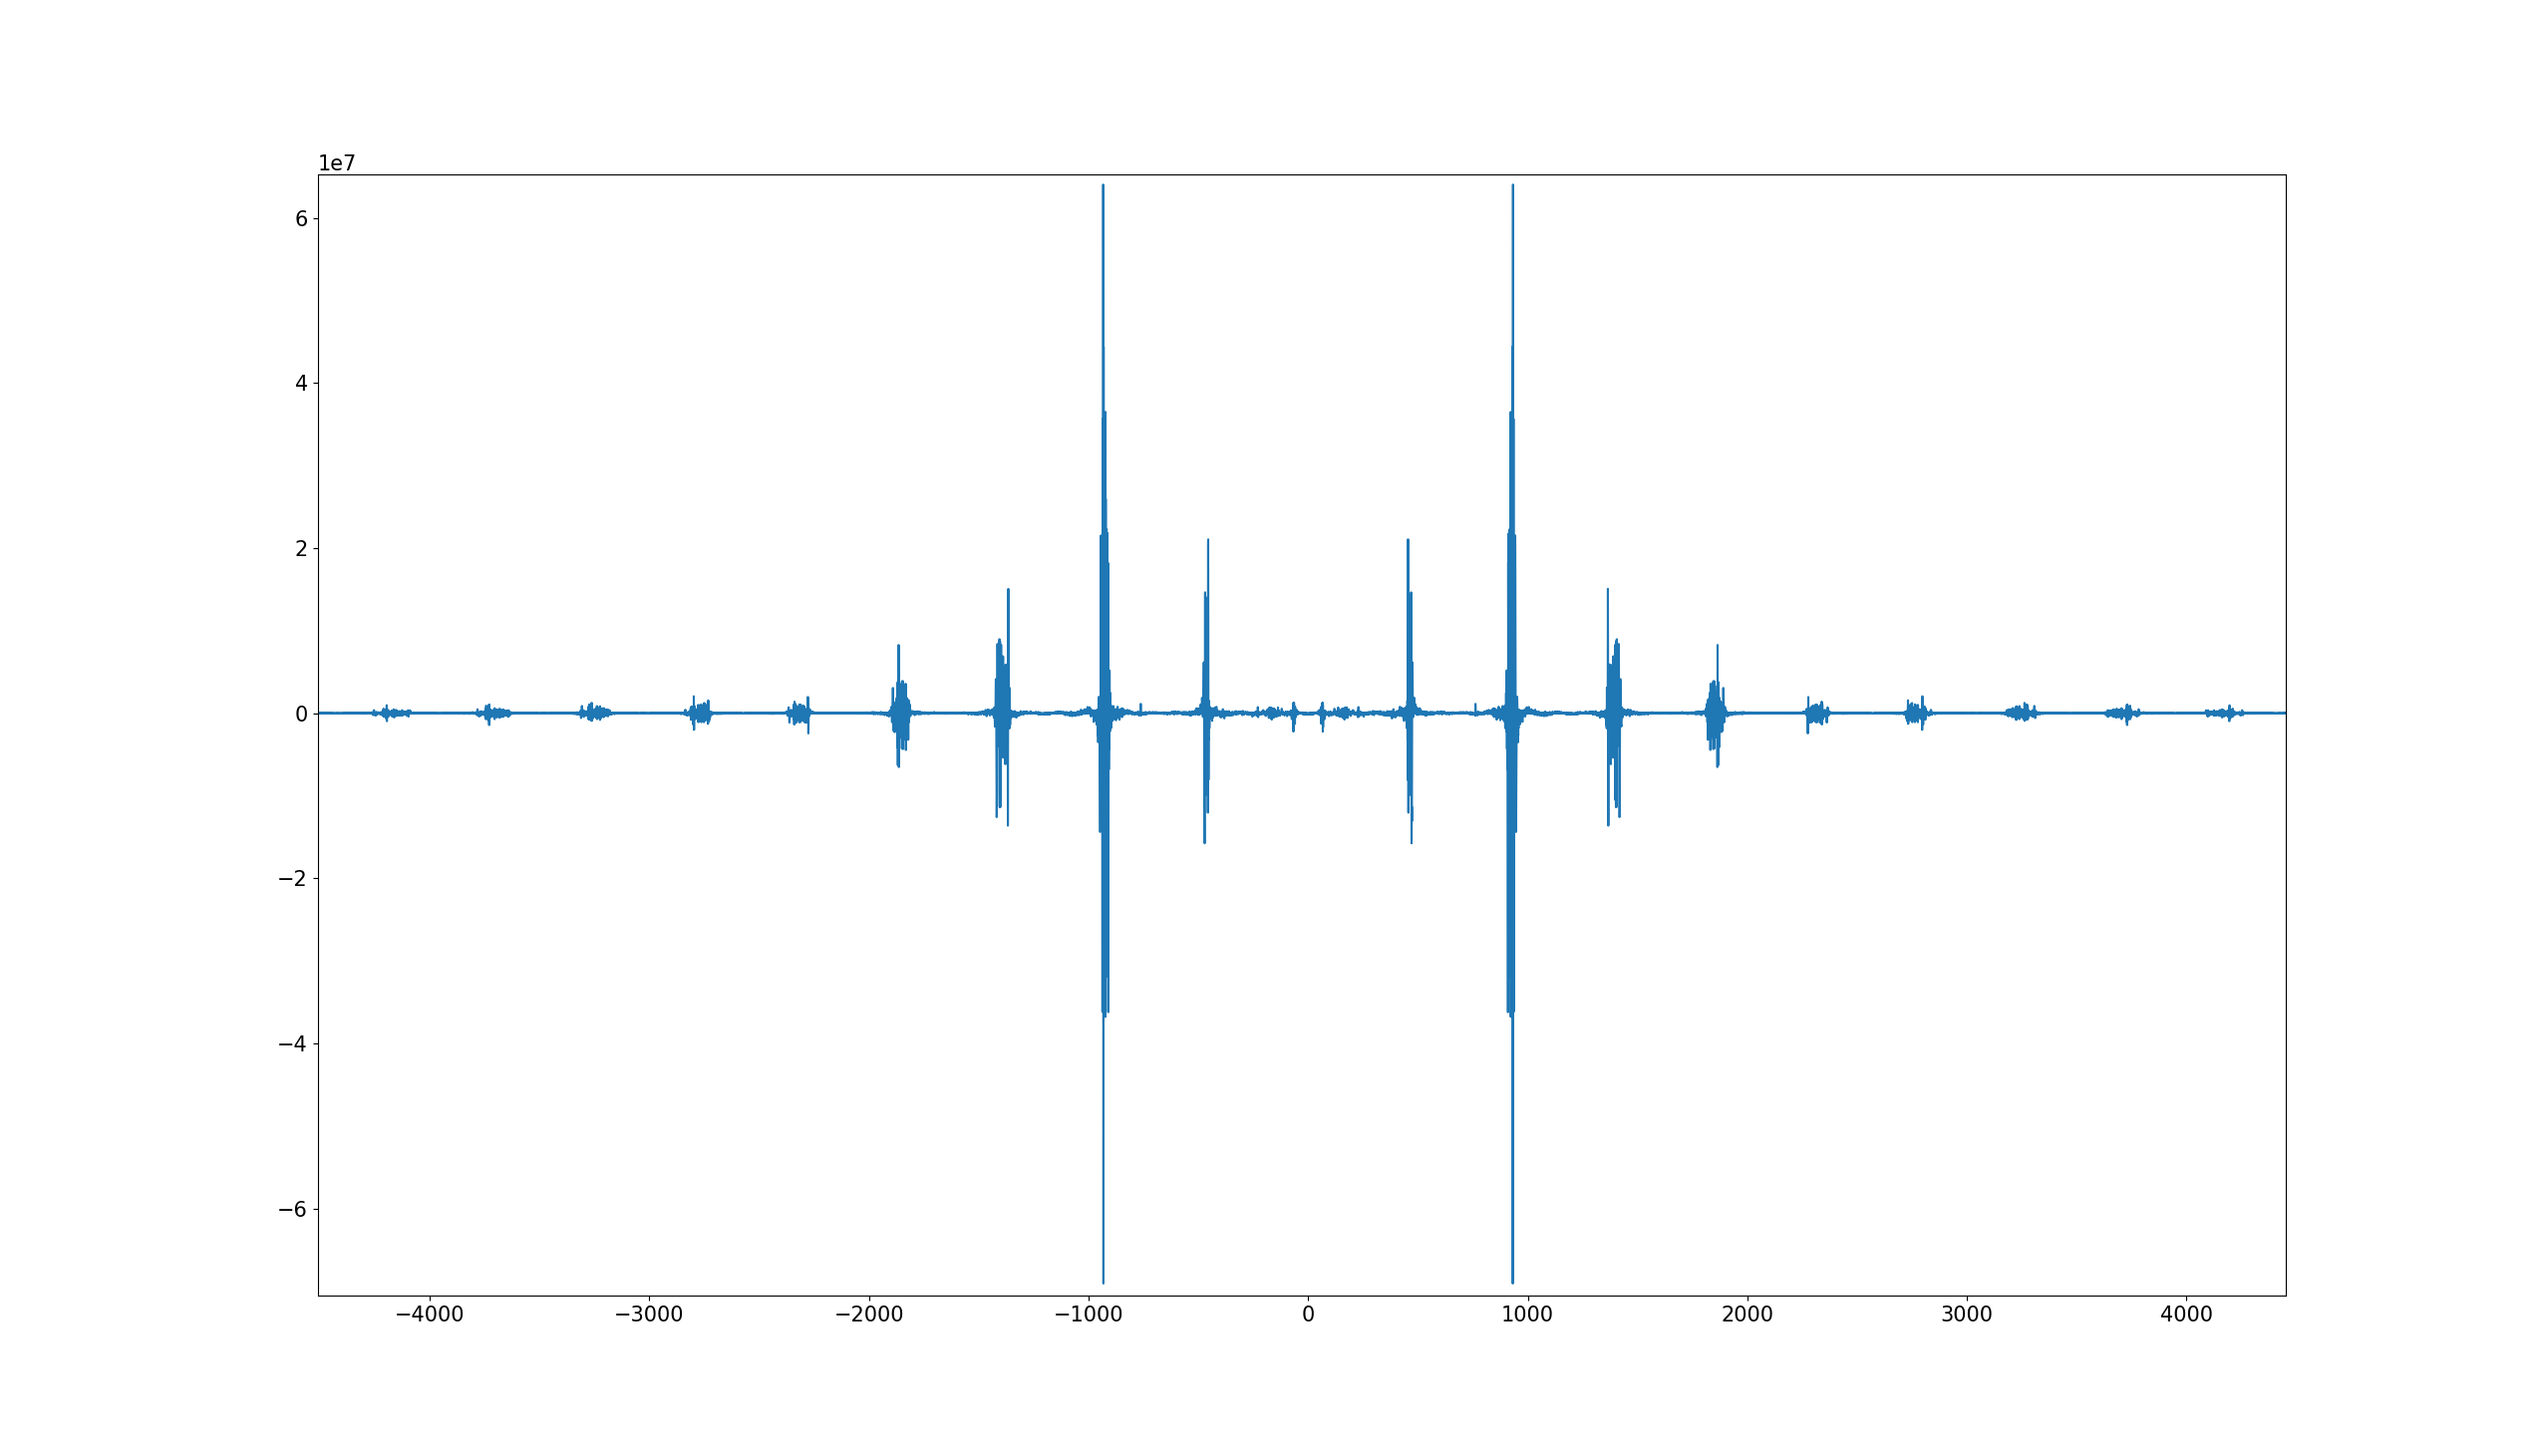
\includegraphics[width=3 in]{../pic/MosquitoSpec.png}
	\caption{The Spectrum Of Mosquitoes Flapping Their Wings}
	\label{fig:MosquitoSpec}
\end{figure}
The fundamental frequency is about $400~\mathrm{Hz}$, if we want to know the instantaneous frequency mosquitoes flap, we only need the fundamental frequency, see Fig.~\ref{fig:FilteredMosquito}.
\begin{figure}[!h]
	\centering
	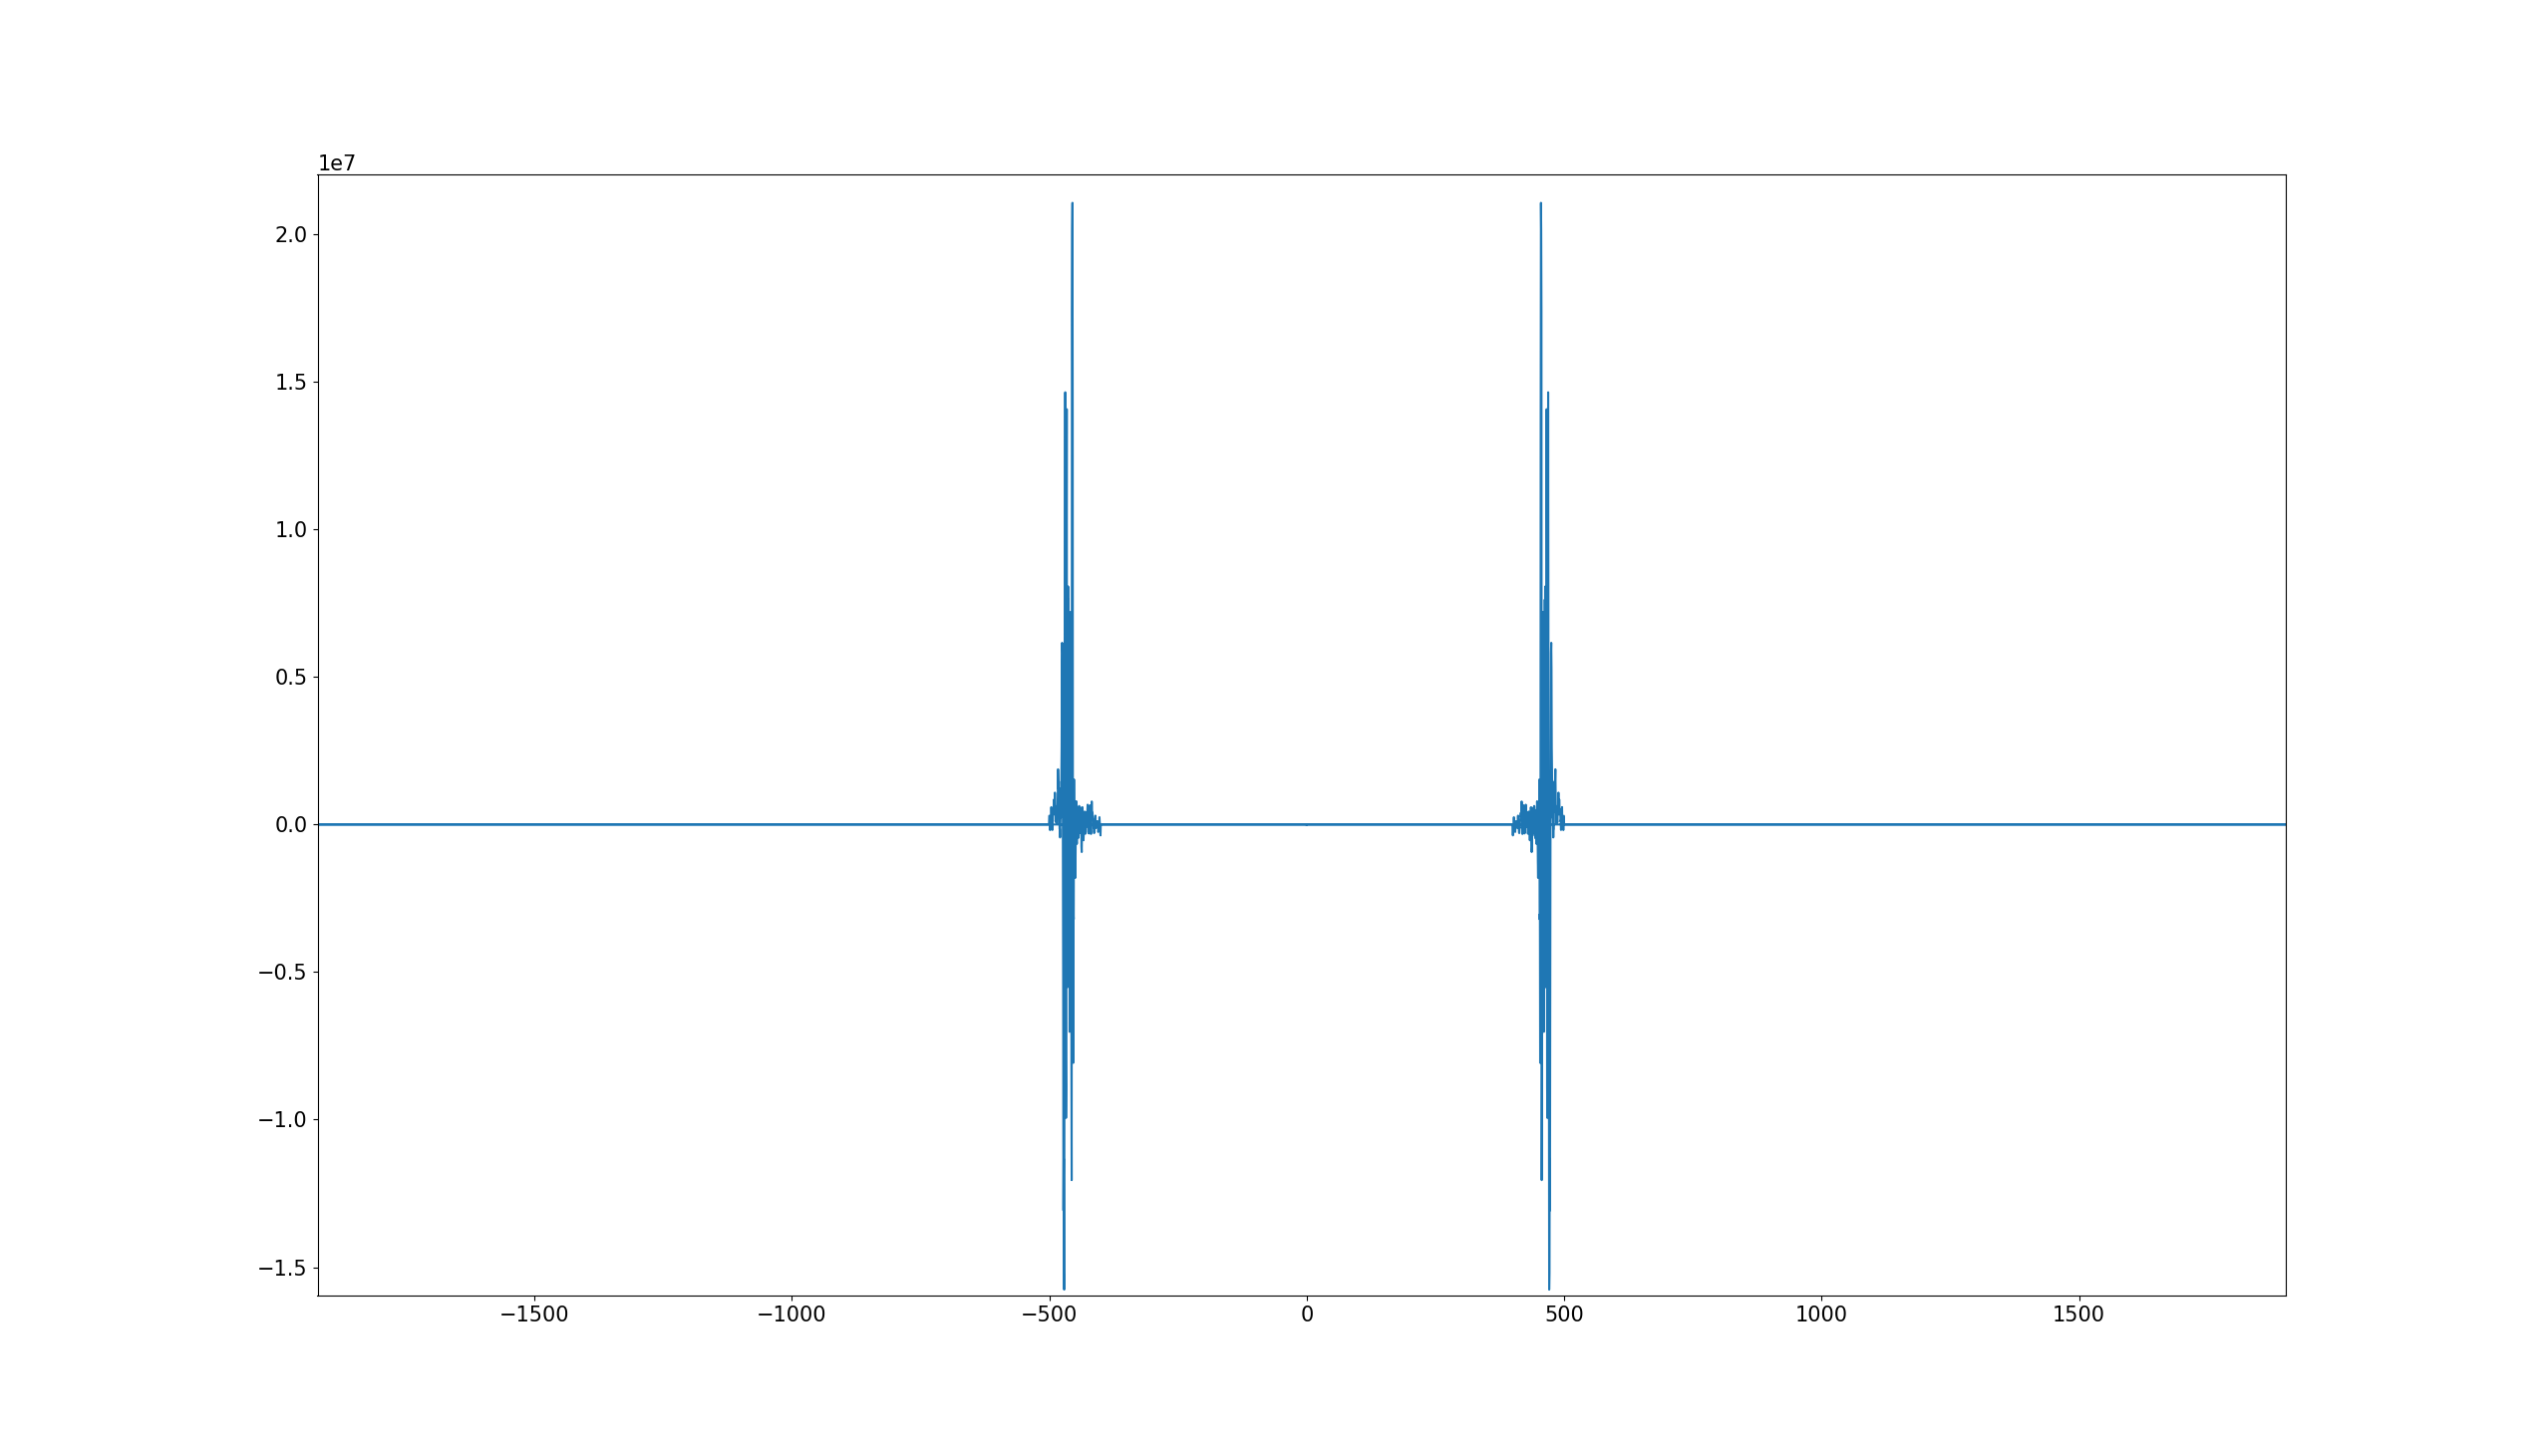
\includegraphics[width=3 in]{../pic/FilteredMosquitoFlap.png}
	\caption{Base-band Spectrum of Mosquitoes' Flapping}
	\label{fig:FilteredMosquito}
\end{figure}

\subsection{Counting With Schmidt Trigger}
To know the instantaneous frequency, I want to cut the wave file into small slice, count how many times the line cross the zero point, and divide this count with the duration time of that small slice to get the frequency here. In order to avoid the detector being too sensitive, I use Schmidt trigger to do this job, see Fig.~\ref{fig:CountFlapping}.

\begin{figure}[!h]
	\centering
	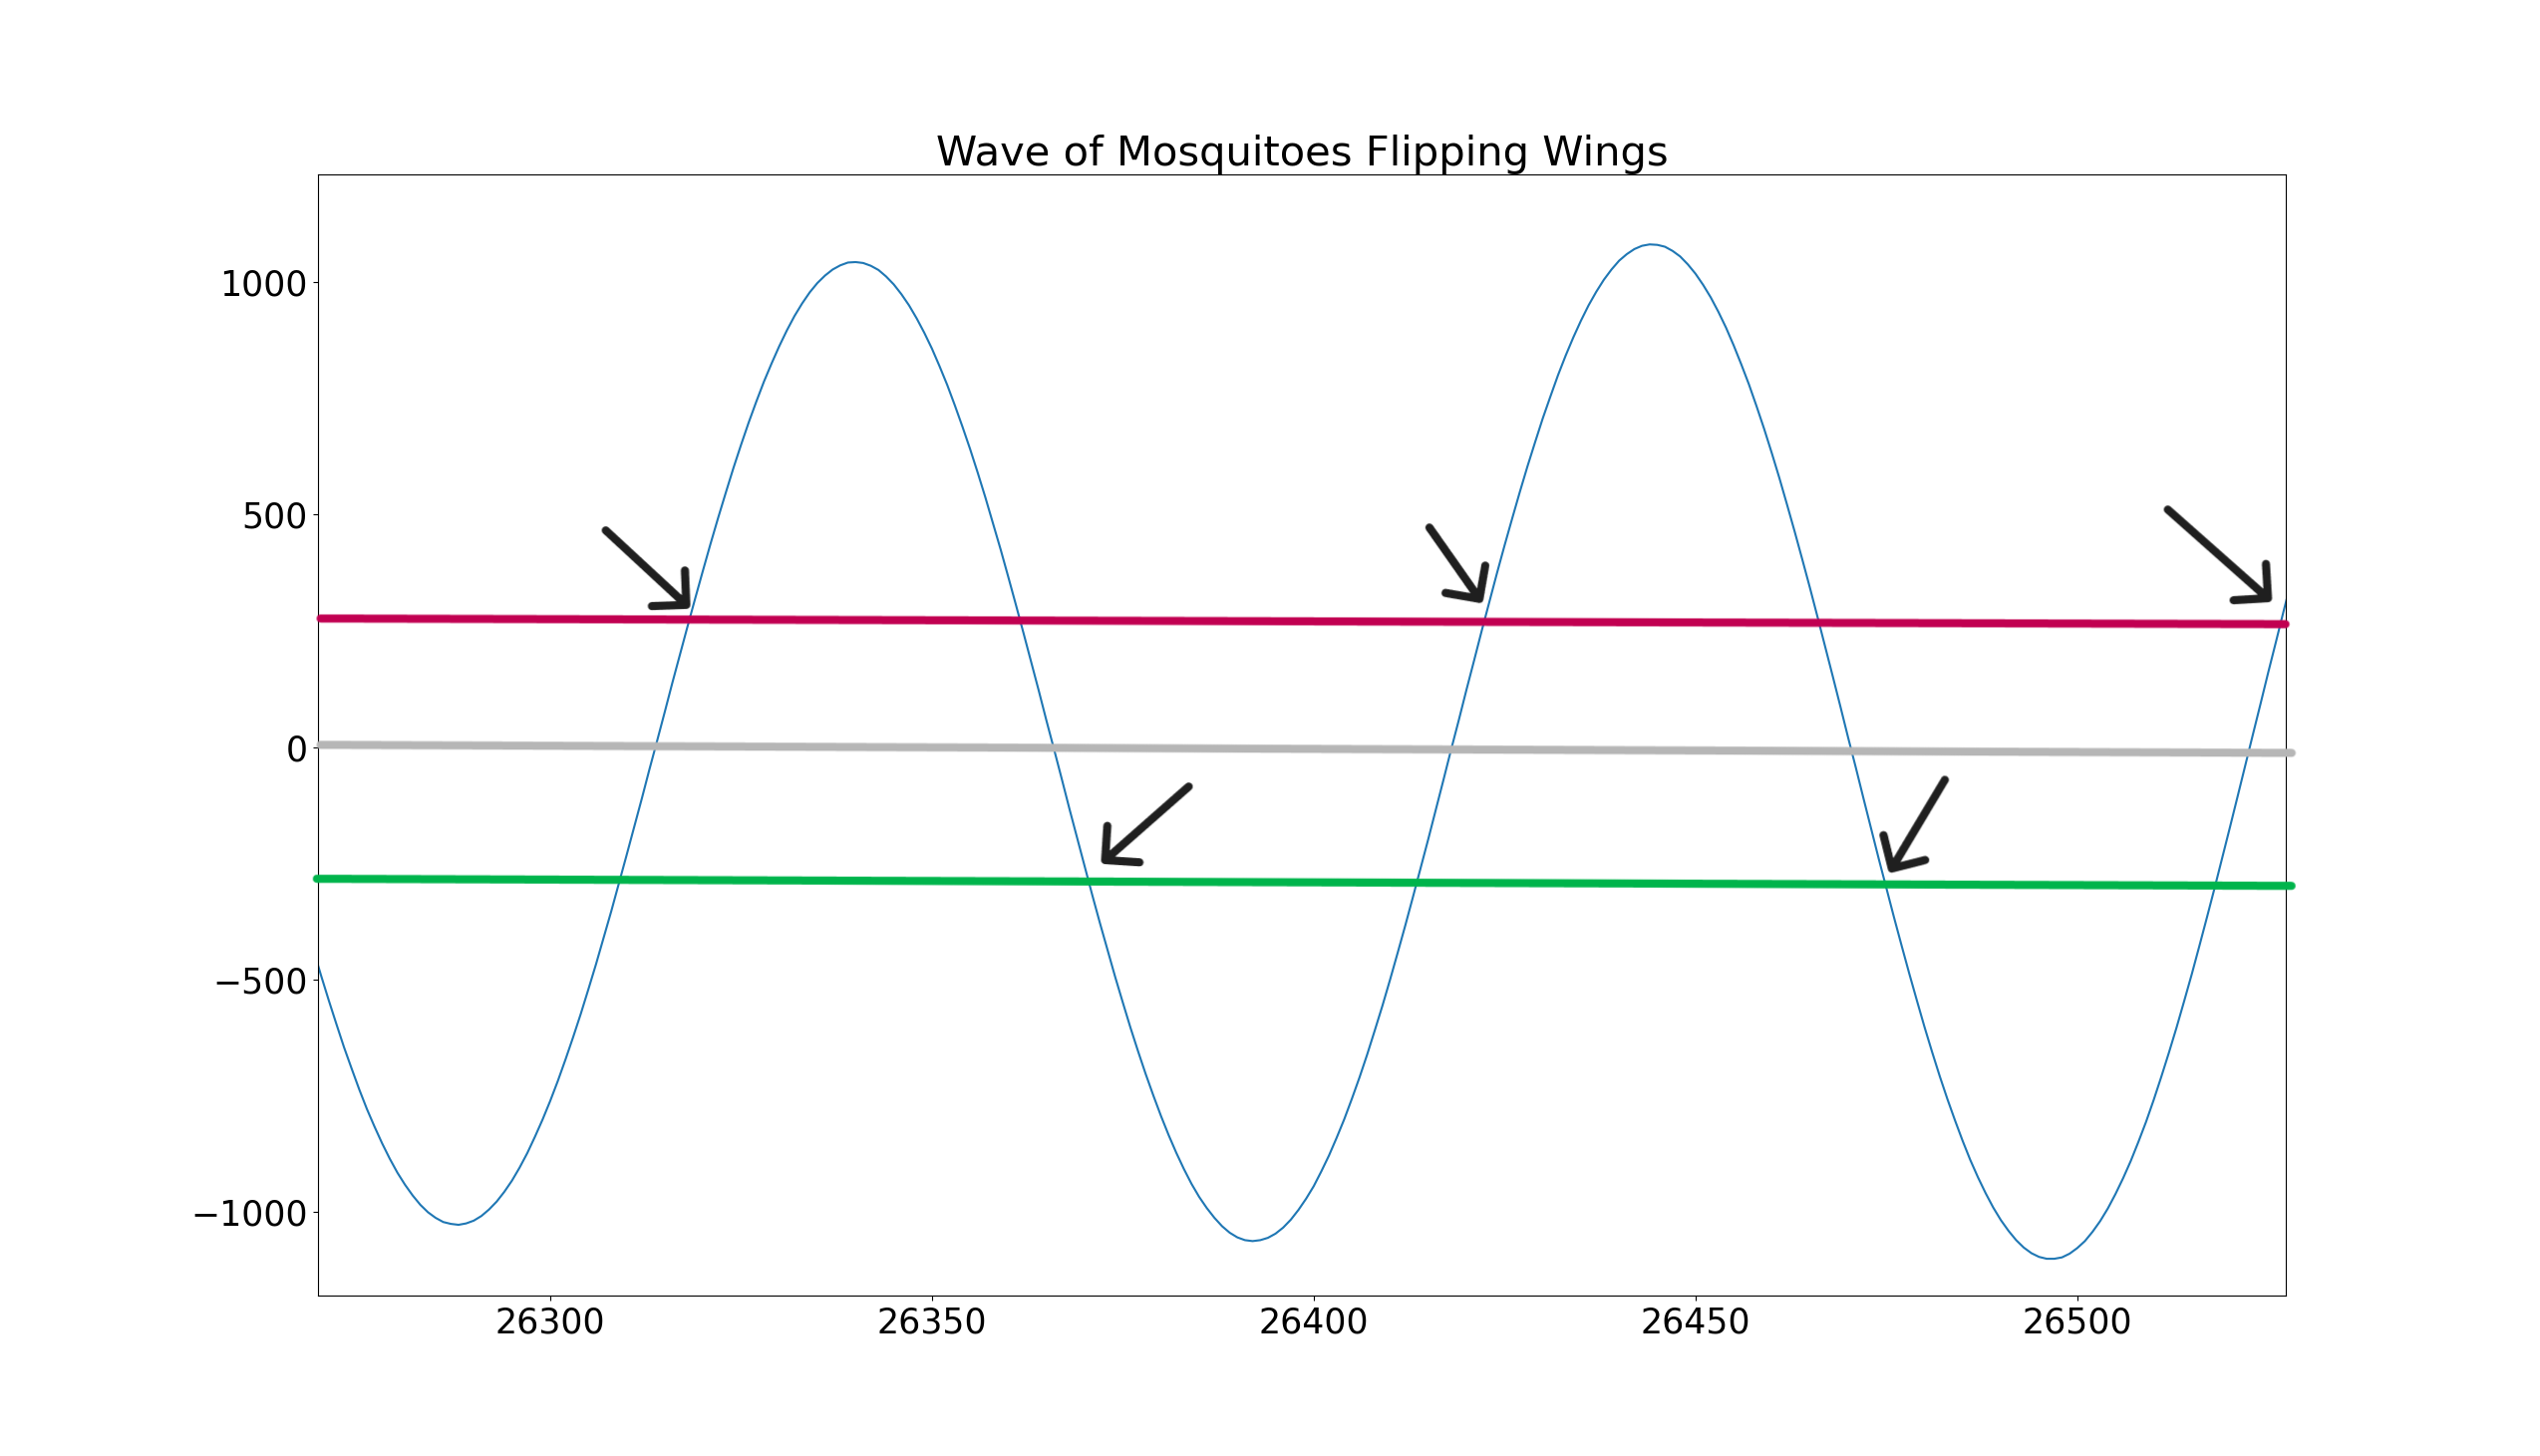
\includegraphics[width=3 in]{../pic/CountFlapping.png}
	\caption{Schmidt Trigger Applied Here}
	\label{fig:CountFlapping}
\end{figure}

\subsection{Results}
Here are my results, see Fig.~\ref{fig:MosquitoResults}.
\begin{figure}[!h]
	\centering
	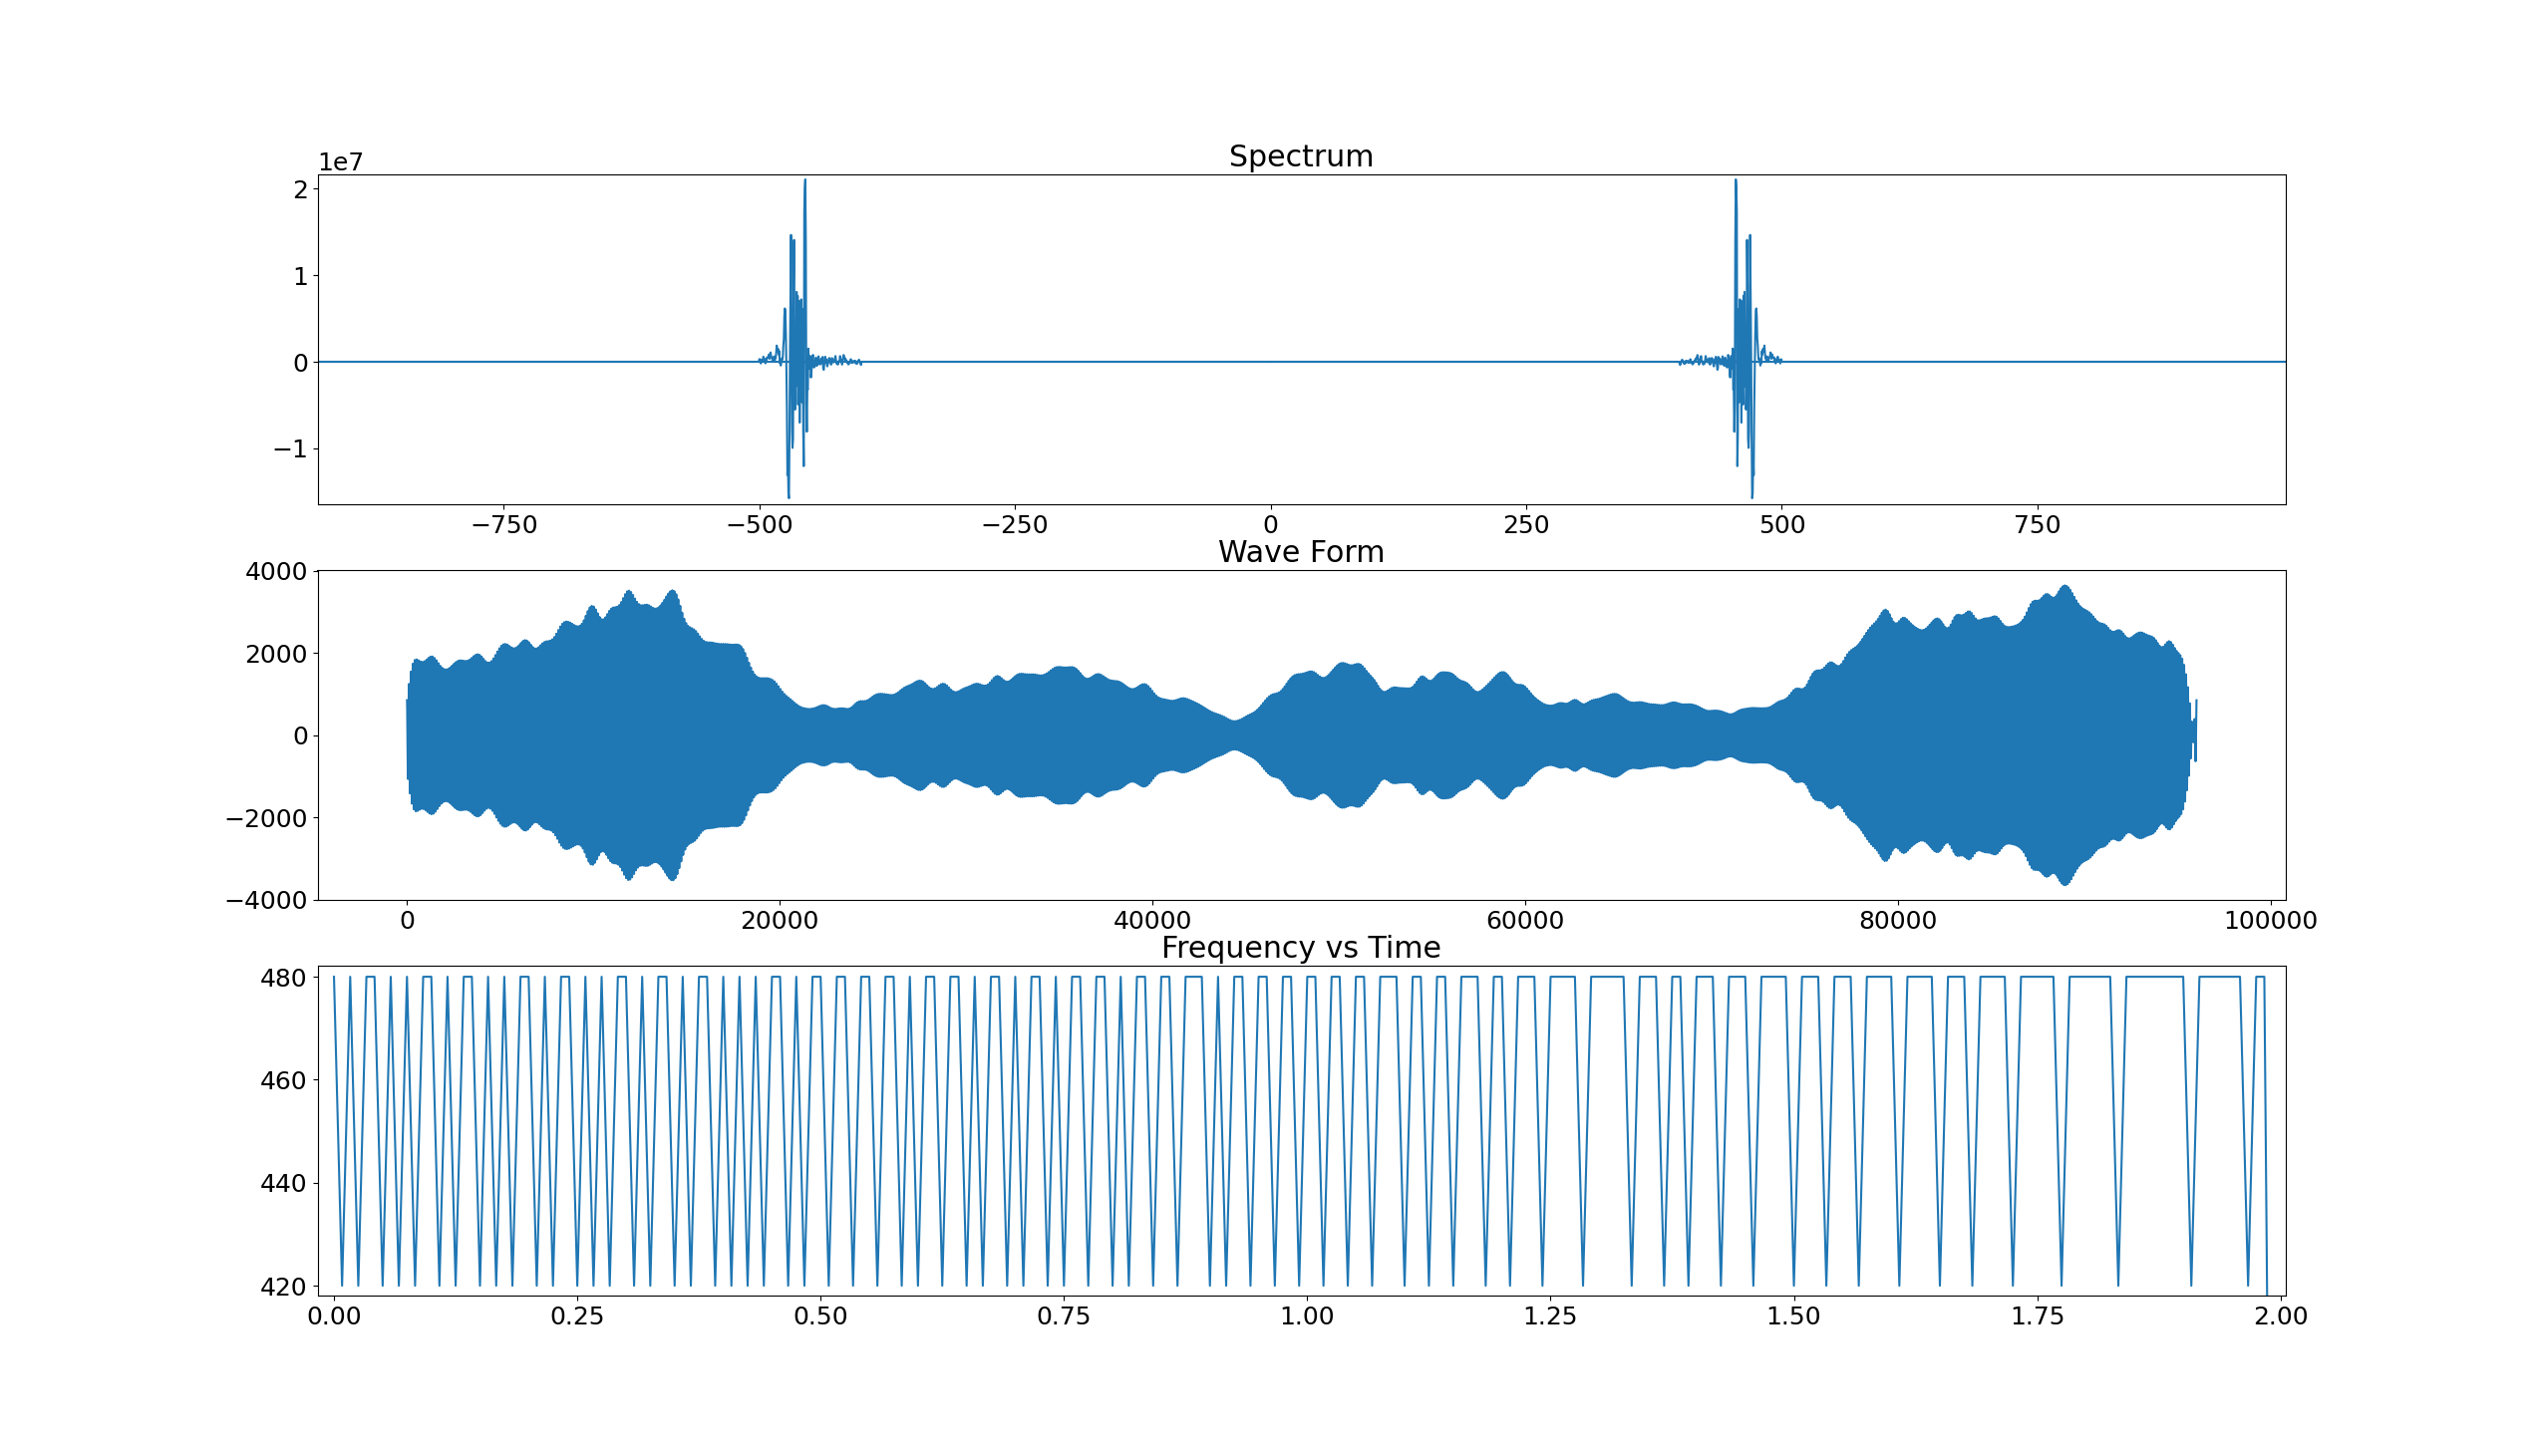
\includegraphics[width=3 in]{../pic/MosquitoResults.png}
	\caption{My Results}
	\label{fig:MosquitoResults}
\end{figure}

\section{Base-band Wireless Communication Simulate}
\subsection{Simulation and Stability Analysis}
I wrote my code by imitating your code, but I made some changes because I thought there might be a problem with the code in class. This mistake will explain the unstable behavior when noise (along with calculation error) is zero. I wrote my comparison in appendix.

In recovery process, we have
\begin{equation}
	\begin{aligned}
		y &= x * h + n \\ 
		\tilde{y} &= \tilde{x} \times \tilde{h} + N_0 \\
	\end{aligned}
\end{equation}
So, the recovered signal $\hat{x}$ is as below
\begin{equation}
	\begin{aligned}
		\mathcal{F}\{\hat{x}\} &= \tilde{y} \times \frac{1}{\tilde{h}} \\  
		&= ( \tilde{x} \times \tilde{h} + N_0 ) \times \frac{1}{\tilde{h}} \\ 
		&= \tilde{x} + \frac{N_0}{\tilde{h}}
	\end{aligned}
	\label{eq:NoiseInXh}
\end{equation}
Here in (\ref{eq:NoiseInXh}), the IIR $N_0/\tilde{h}$ , is why $\hat{x}$ can be unstable.

\subsection{Unstable Behavior When Noise is Zero}
In mathematics, it is impossible to see unstable behavior in (\ref{eq:NoNoiseXh}).
\begin{equation}
	\begin{aligned}
		\mathcal{F}\{\hat{x}\} &= \tilde{y} \times \frac{1}{\tilde{h}} \\  
		&= ( \tilde{x} \times \tilde{h}) \times \frac{1}{\tilde{h}} \\ 
		&= \tilde{x}
	\end{aligned}
\label{eq:NoNoiseXh}
\end{equation}
So, there must be other noise in the code. What I found is that there will be a very small error in division of python, and it is exactly this little error that makes $1/\tilde{h}$ to oscillate infinitely.

Please see the terminal output in Fig.~\ref{fig:CalculationError} which proves my guess.
\begin{figure}[!h]
	\centering
	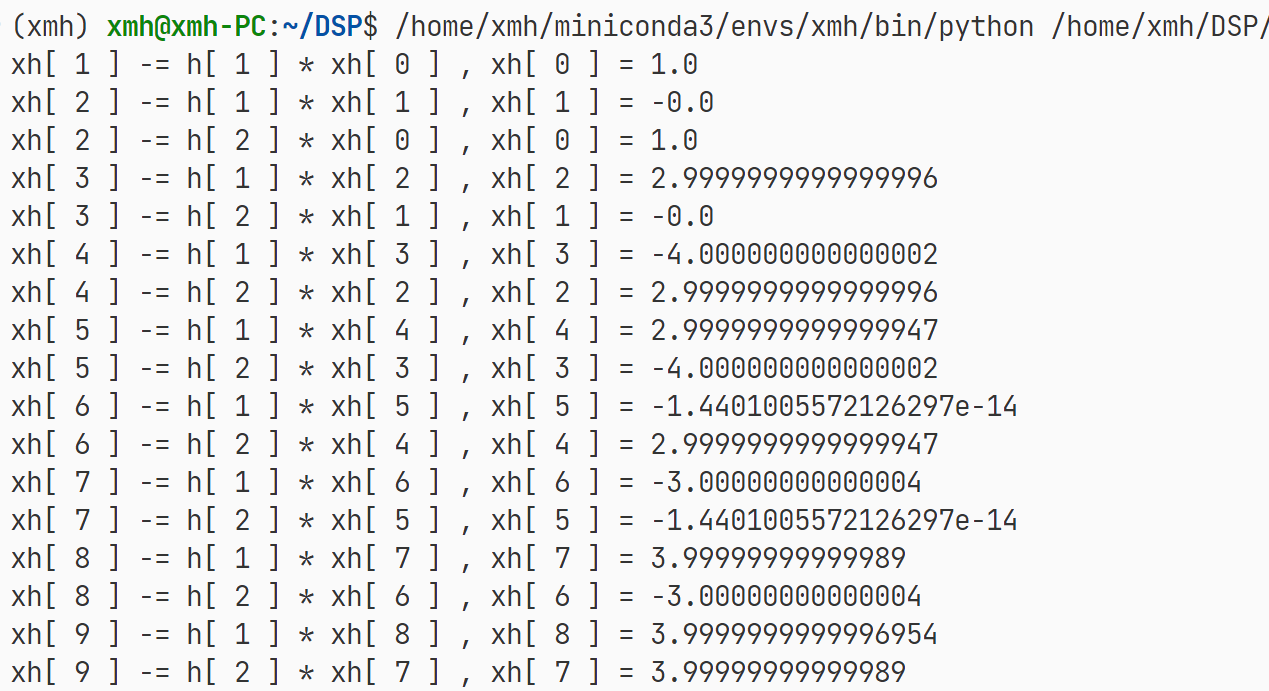
\includegraphics[width=3 in]{../pic/CalculationError.png}
	\caption{Error in Division Calculation}
	\label{fig:CalculationError}
\end{figure}

This error is revealed in float numbers like $2.99\cdots96$ and $-4.00\cdots02$ in line 4 and 6 of Fig.~\ref{fig:CalculationError}.

There are my comparison between whether there is noise or calculation error in signal $y$, see Fig.~\ref{fig:Comparison}.

% \newpage

\begin{figure}[!h]
	\centering
	\subfigure[$\tilde{h}$ is stable]{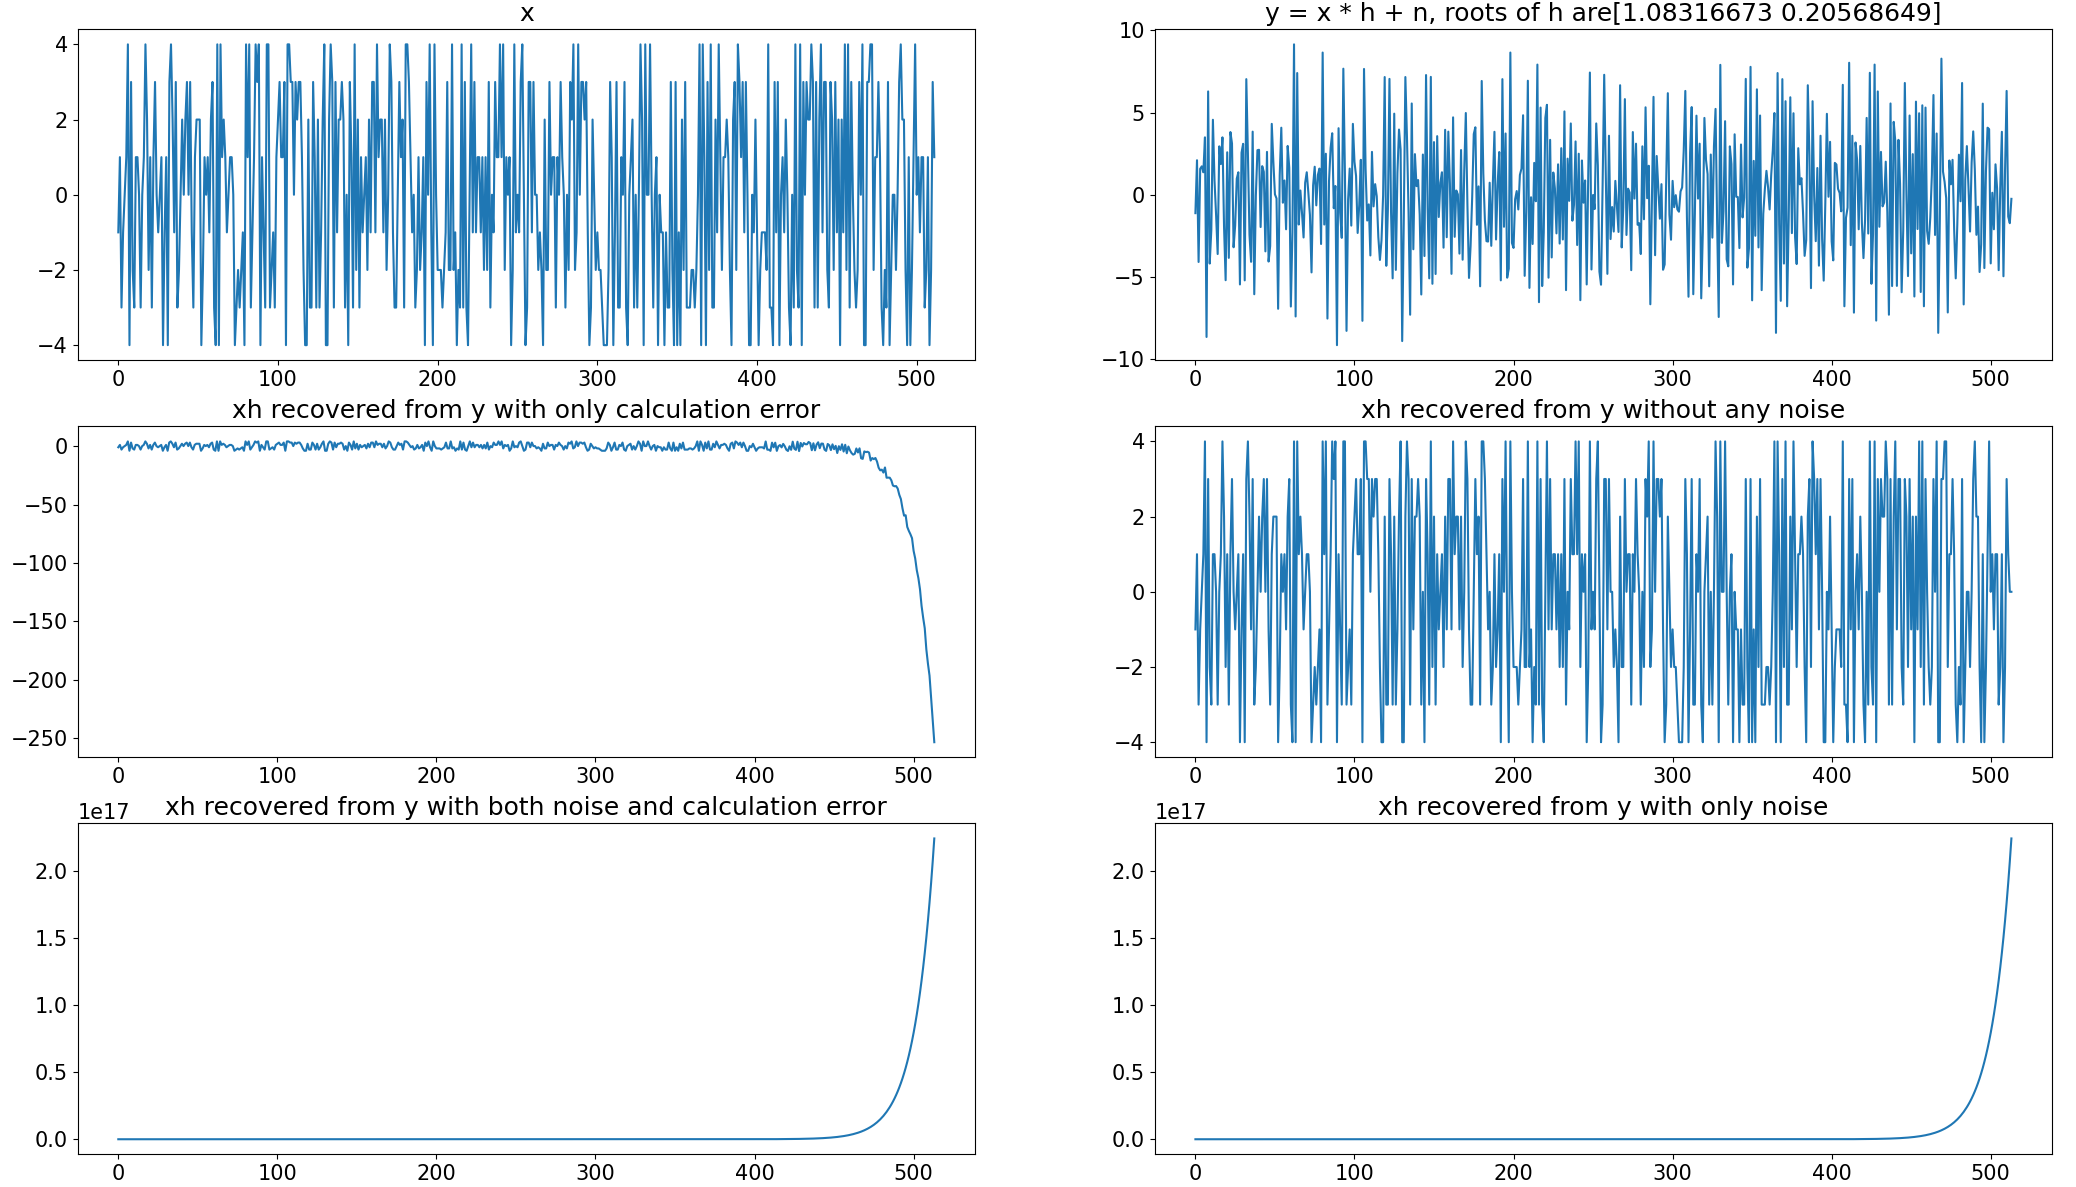
\includegraphics[height=1.7 in]{../pic/StabilityComparison.png}
	\label{fig:StabilityComparison}}
	\hspace{0 pt}
	\subfigure[$\tilde{h}$ is unstable]{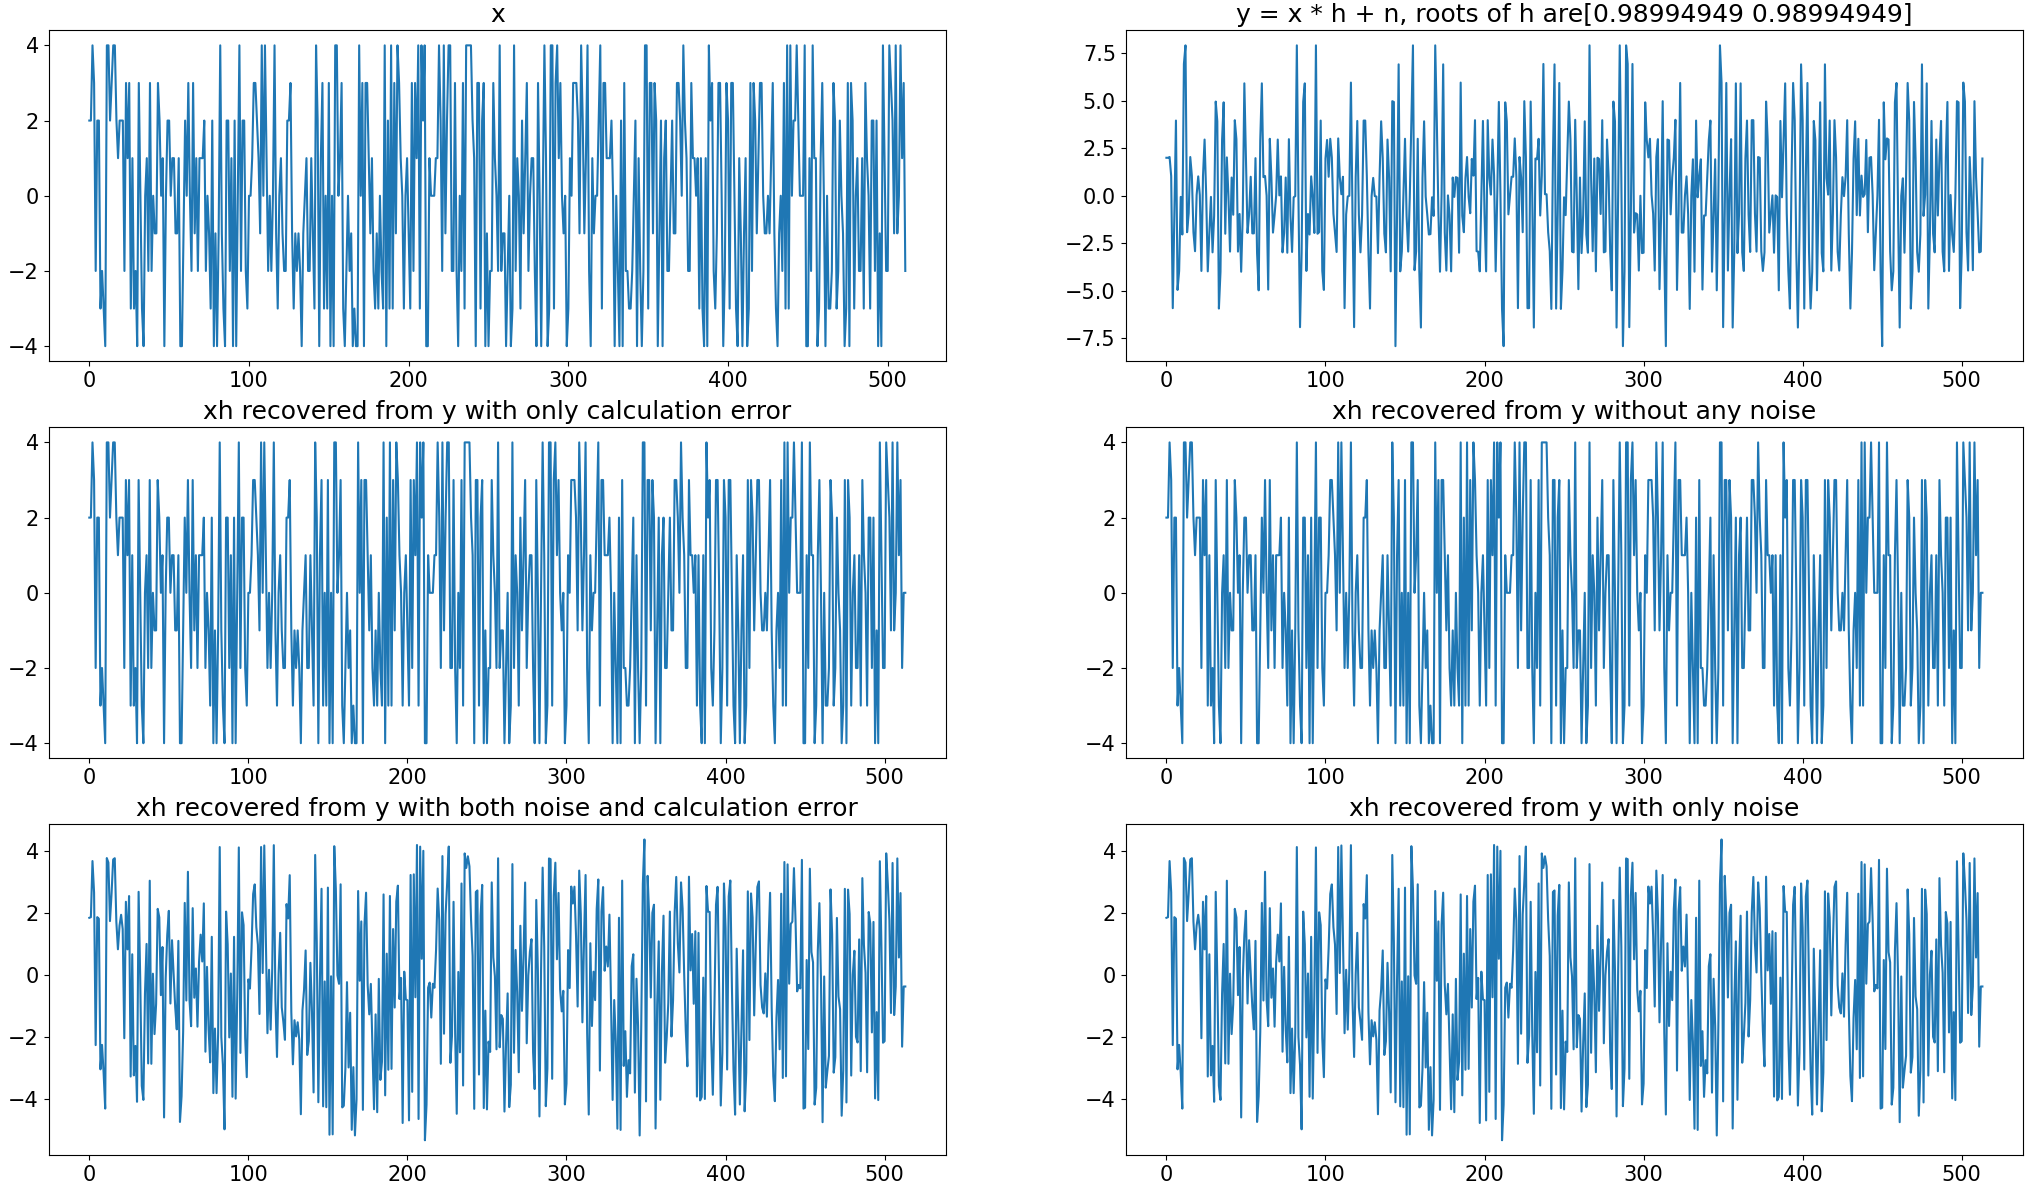
\includegraphics[height=1.7 in]{../pic/AllStableComparison.png}
	\label{fig:AllStableComparison}}
	\caption{Stability Comparison when $\tilde{h}$ is different}
	\label{fig:Comparison}
\end{figure}

We can see in Fig.~\ref{fig:StabilityComparison} that when $\tilde{h}$ is unstable, $\hat{x}$ recovered from y only with calculation error went infinite, but $y$ without both calculation error and noise can be perfectly recovered. This phenomenon is because unstable amplified the noise or the calculation error in recovery, so if there's no disturb in $y$, it is possible to recover the original signal $x$.

Also, when $\tilde{h}$ is stable or is decrement oscillation, the noise and the calculation error will be decreasing along with the recovery process, so without noise is no longer a necessary condition for signal recovery. However, in this condition, only $y$ without any noise can be perfectly recovered ($\hat{x} = x$).

\bibliographystyle{ieeetr}
\bibliography{../bib/database}

\begin{appendices}
\section{Possible Mistakes in Lesson}
Dear Yi, I may found a small mistake in your code on Tuesday's (Dec.6) lesson. It is about the recovering of
from $y = x * h$. 

Please see the probably incorrect code as below:
\begin{python}
def reX_estimate(y, h):
	N = len(y)
	M = len(h)
	print("Length of y is ", N,", Length of h is ", M)
	xh = y.copy()
	for n in range(N):
		print("Info: n is now ", n)
		for m in range(1, min(M, n)): # Mistake here, n should be n + 1
			xh[n] -= h[m] * xh[n - m]
			print("xh[", n,"] -= h[",m,"] * xh[",n - m,"]")
		xh[n] /= h[0]
	return xh
\end{python}

The length of $h$ is $3$ and the roots of $h$ are about $[1.77, 0.57]$. Key point is in the output, see Fig.~\ref{fig:output}.

\begin{figure}[!h]
	\centering
	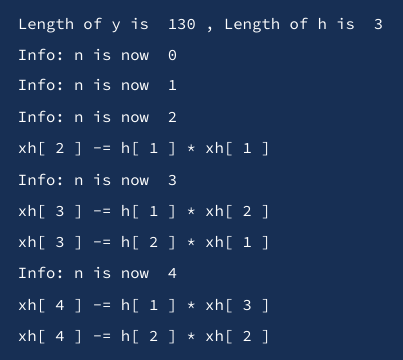
\includegraphics[width=2 in]{../pic/comparisonOutput.png}
	\caption{Output of Test Code}
	\label{fig:output}
\end{figure}

We can find that while $\hat{x}[2] = y[2] = h[0] \times x[2] + h[1]\times x[1] + h[2] \times x[0]$ , this code only minus $h[1] \times x[1]$, that is the small mistake.

This small mistake in recovering $x$ is \emph{working as noise}, as a result, the $h(n)$ which is an unstable IIR, will \emph{amplify this noise} and finally cause the \emph{unstable behavior}. As the Fig.~\ref{fig:diffRec} revealed.

\begin{figure}[!h]
	\centering
	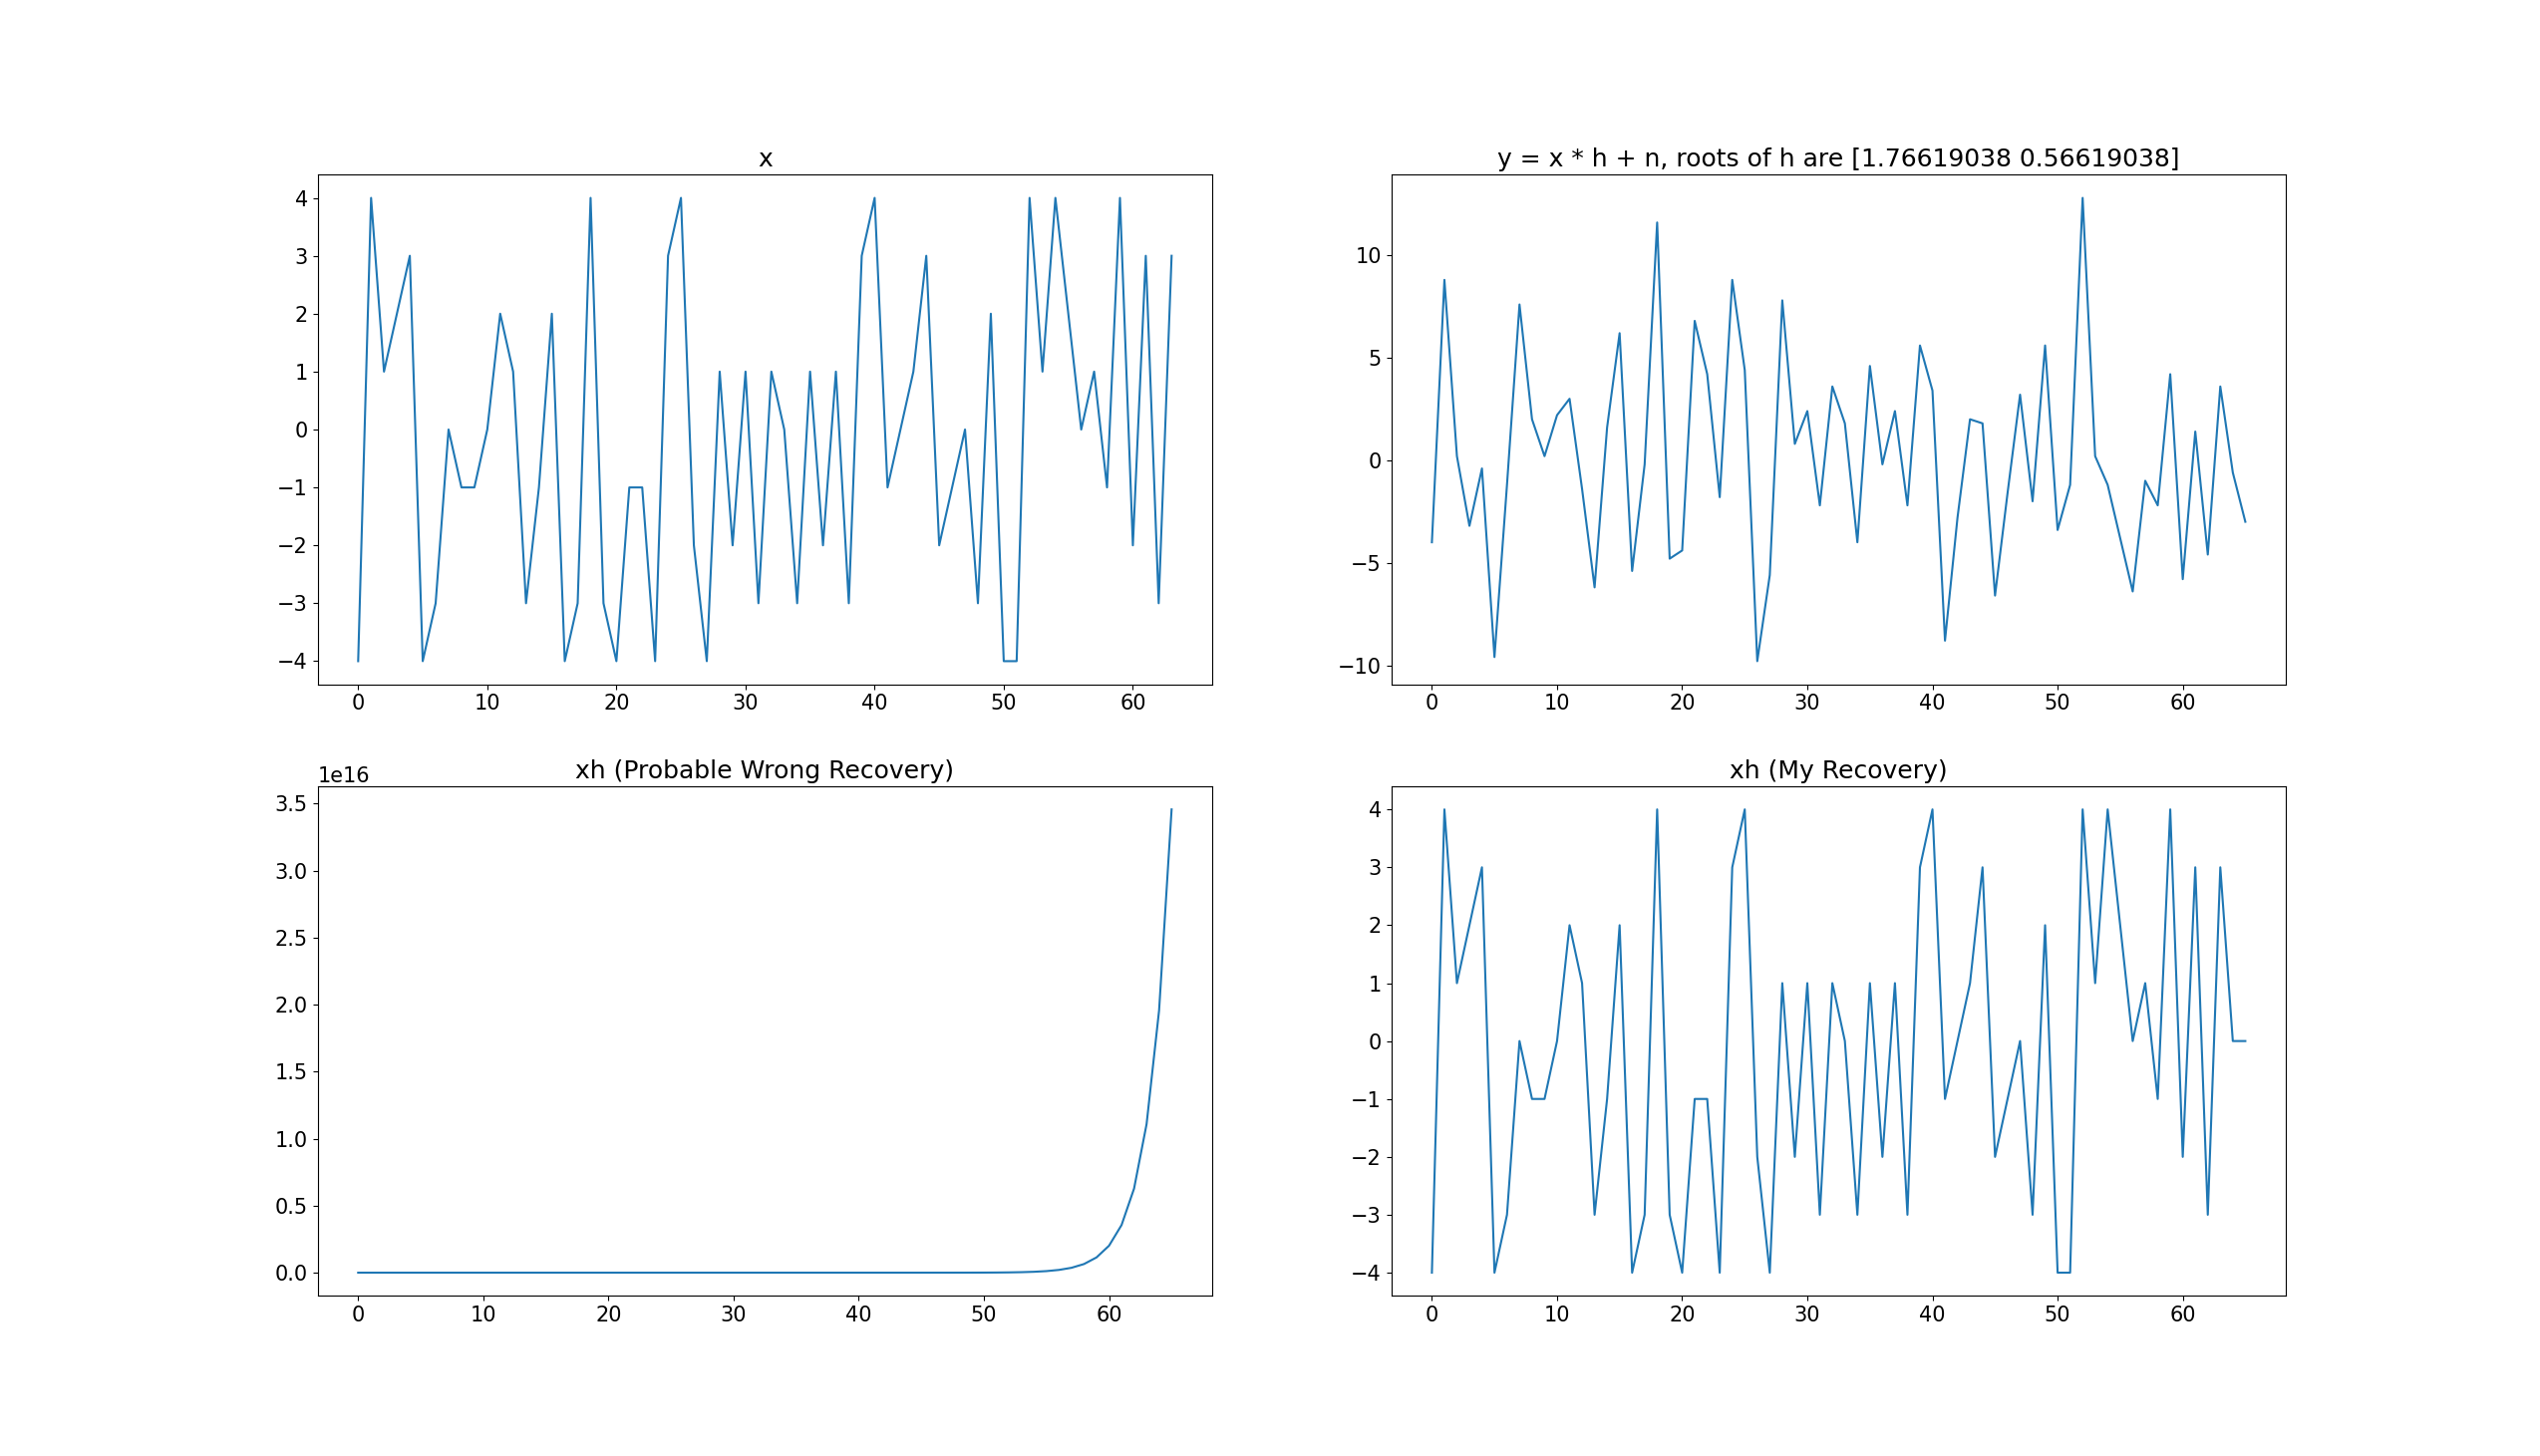
\includegraphics[width=6 in]{../pic/diffRec.png}
	\caption{Different Behavior Between Previous Code and Current Code}
	\label{fig:diffRec}
\end{figure}

\newpage

\section{Code Listing}
\begin{python}
# simulate.py
import numpy as np
import matplotlib.pyplot as plt
plt.rcParams.update({'font.size': 15})

def genPAM(N, M):
    """Generate PAM Signal"""
    return (np.random.randint(-M, M + 1, (N)))

def genNoise(y, snr = 20):
    """Generate White Noise"""
    Es = np.mean(y**2)
    sigma = np.sqrt(Es / 10 ** ( snr / 10))
    n = sigma * np.random.randn(len(y))
    return n + y, n

def reX_estimate(y, h, ErrorFlag=1):
    """Estimate x From y"""
    N = len(y)
    M = len(h)
    xh = y.copy()
    for n in range(N):
        # print("Info: n is now ", n)
        for m in range(1, min(M, n + 1)):
            xh[n] -= h[m] * xh[n - m]
            # if ErrorFlag and n <= 20:
            #     print("xh[", n,"] -= h[",m,"] * xh[",n - m,"]", ", xh[", n - m,"] =",xh[n - m])
        xh[n] /= h[0]
        if ErrorFlag == 0:
            xh[n] = np.round(xh[n], 8) #Exclude Error generated by calculation accuracy
    return xh

#parameters
N = 256
Nc = 3
M = 4

#generate x and h randomly
x = genPAM(N, M)
h = np.random.randn(Nc)
# h = [1, 0, -0.98]

#generate y as received signal
y = np.convolve(x, h)
yn, n = genNoise(y, snr = 30) 

#recover x in different methods
xh = reX_estimate(y, h)
xh_new = reX_estimate(y, h, ErrorFlag=0)
xhn = reX_estimate(yn, h)
xhn_new = reX_estimate(yn, h, ErrorFlag=0)

#draw the results and the comparison
fig = plt.figure(figsize=(12, 8))

ax = fig.add_subplot(3, 2, 1)
ax.plot(x)
ax.set_title('x')
ax = fig.add_subplot(3, 2, 2)
ax.set_title('y = x * h + n, roots of h are' + str(np.abs(np.roots(h))))
ax.plot(y)
ax = fig.add_subplot(3, 2, 3)
ax.set_title('xh recovered from y with only calculation error')
ax.plot(xh)
ax = fig.add_subplot(3, 2, 4)
ax.set_title('xh recovered from y without any noise')
ax.plot(xh_new)
ax = fig.add_subplot(3, 2, 5)
ax.set_title('xh recovered from y with both noise and calculation error')
ax.plot(xhn)
ax = fig.add_subplot(3, 2, 6)
ax.set_title('xh recovered from y with only noise')
ax.plot(xhn_new)

plt.show()

\end{python}

\begin{python}
# Mosquito.py
from scipy.io.wavfile import read, write
import numpy as np
from numpy.fft import fft, fftfreq, ifft
from matplotlib import pyplot as plt
plt.rcParams.update({'font.size': 18})

def loadWAV(fname):
    fs, w = read(fname)
    sec = len(w)/fs
    wt = fft(w)
    freq = fftfreq(wt.size, d=1/fs)
    """Simple High-Pass Filter"""
    fl = 400
    wt[int(-fl * sec):] = 0
    wt[:int(fl * sec)] = 0
    """Simple Low-Pass Filter"""
    fh = 500
    cfq = wt.size/2
    wt[int(cfq - (fs/2 - fh) * sec):int(cfq + (fs/2 - fh) * sec)] = 0
    return fs, w, wt, freq

def countFlap(w, fs, gate, intv):
    N = len(w)
    M = N//intv
    count = 0
    L = np.zeros(M)
    if w[0] > 0:
        flag = 1
    else:
        flag = -1
    for n in range(M):
        for m in range(intv):
            index = int(intv * n + m)
            if flag * w[index] > -gate:
                pass
            else:
                count += 1
                flag = w[index] / np.abs(w[index])
        L[n] = count/2
        count = 0
    return intv/fs, L

fs, w, wt, freq = loadWAV("/home/xmh/DSP/projF/code/mosquito-cut.wav")
iw = np.array(np.real(ifft(wt)), dtype=np.int16)
write('/home/xmh/DSP/projF/code/mosquito-out.wav', fs, iw)

dt, L = countFlap(iw, fs, gate=300, intv=400)
F = L/(dt)
gapTime = np.arange(0, 2, dt)

fig = plt.figure(figsize=(12, 8))

ax = fig.add_subplot(311)
ax.set_title("Spectrum")
ax.plot(freq, np.real(wt))

ax = fig.add_subplot(312)
ax.set_title("Wave Form")
ax.plot(iw)

ax = fig.add_subplot(313)
ax.set_title("Frequency vs Time")
ax.plot(gapTime, F)

plt.show()
\end{python}

\end{appendices}

\end{document}